\documentclass[a4paper]{article}
\usepackage{color}              %Farben, f.r \definecolor{}
\usepackage{amssymb}            %Mathematische Symbole
\usepackage{amsthm}             %Besseres \newtheorem
\usepackage{amsmath}           %Mathematische Umgebungen
\usepackage{mathtools}          %\xRightarrow, etc
\usepackage{mathrsfs}           %enthaelt \mathscr
\usepackage{graphicx}
\usepackage{enumerate}          % in-place numerations def.
\usepackage{fullpage}

\usepackage{array}
%\usepackage{multicol}
%\usepackage[notref,notcite]{showkeys}
%\usepackage{algorithm,algorithmic}
\usepackage{color}

\usepackage{graphicx}
\usepackage{xypic}
\entrymodifiers={+!!<0pt,\fontdimen22\textfont2>}
\usepackage[all]{xy}

\usepackage{float}
\usepackage{tikz}
\usepackage{tikz-cd}
\usepackage{tikz,fullpage}
\usetikzlibrary{arrows,%
                petri,%
                topaths}%
\usepackage{tkz-berge}
\usepackage[position=top]{subfig}
\usetikzlibrary{shapes.geometric}
\usetikzlibrary{decorations.markings}
\usetikzlibrary{graphs}

\newtheoremstyle{myremark} % name
    {7pt}                    % Space above
    {7pt}                    % Space below
    {}  	                 % Body font
    {}                           % Indent amount
    {\bf}       	         % Theorem head font
    {.}                          % Punctuation after theorem head
    {.5em}                       % Space after theorem head
    {}  % Theorem head spec (can be left empty, meaning ‘normal’)

\theoremstyle{plain}
\newtheorem{lemma}{Lemma}
\newtheorem{theorem}[lemma]{Theorem}
\newtheorem{fact}[lemma]{Fact}
\newtheorem{definition}[lemma]{Definition}
\newtheorem{corollary}[lemma]{Corollary}
\newtheorem{proposition}[lemma]{Proposition}
\newtheorem{conjecture}[lemma]{Conjecture}
\newtheorem{observation}[lemma]{Observation}
\newtheorem{problem}[lemma]{Problem}
\newtheorem{notation}[lemma]{Notation}
\newtheorem*{claim}{Claim}

\theoremstyle{myremark}
\newtheorem{remark}[lemma]{Remark}
\newtheorem{example}[lemma]{Example}

%%%%%% EDIT HERE: %%%%%%%%%%%
\newcommand{\LECTURENUMBER}{0}
\newcommand{\LECTURETITLE}{Short title}
\newcommand{\LECTURESCRIBE}{Your name}

%% Dokument Beginn %%%%%%%%%%%%%%%%%%%%%%%%%%%%%%%%%%%%%%%%%%%%%%%%%%%%%%%%
\begin{document}
\thispagestyle{empty}

\begin{center}
	{\Large\bf Graph coloring}\\
	{\bf Lecture notes, vol. 7, \\ The chromatic polynomial}\\
\end{center}
Lecturer: Michal Adamaszek \hfill Scribe: Mortan J. Thomsen
\begin{center}
\line(1,0){450}
\end{center}

%%%%%%% EDIT ALSO BELOW: %%%%%%%%%%%%%%%%

\noindent Further on planar graphs. In the 1930s Birkhoff and Whitney had the idea to, instead of constructing one $4$-colouring for a planar graph, rather count all $4$-colourings, and determine whether the result is $>0$. This leads to the notion of the chromatic polynomial.
\begin{definition} For a graph $G$ we define the chromatic function $P_G(t)$, $P(G,t)$ or $P(t)$, as 
\begin{align*}
P_G(t)&=\#\text{ of vertex colourings of G with colours }\lbrace 1,\dots ,t\rbrace\\
&=\left|\left\lbrace c:V(G)\to \lbrace 1,\dots ,t\rbrace : c\text{ is a colouring}\right\rbrace\right|
\end{align*}
\end{definition}
\begin{example}
\begin{enumerate}
\item[$\circ$] $G=\overline{K_n}$, $P_G(t)=t^n$.
\item[$\circ$] $G=K_n$, $P_G(t)=t(t-1) \cdots (t-(n-1))$.
\begin{center}
\begin {tikzpicture}

\draw   
           node[fill,circle,inner sep=0pt,minimum size=3pt] (n1) at (0,0) {}
           (0,0) node [text=black,left] {$t-3$}
	node[fill,circle,inner sep=0pt,minimum size=3pt] (n2) at (1,0) {}
	(1,0) node [text=black,right] {$t-2$} 
	node[fill,circle,inner sep=0pt,minimum size=3pt] (n3) at (0,1) {} 
	(0,1) node [text=black,left] {$t$}
	node[fill,circle,inner sep=0pt,minimum size=3pt] (n4) at (1,1) {}
	(1,1) node [text=black,right] {$t-1$}
[line width = 1 pt, black, -] (n1) edge (n4)
[line width = 1 pt, black, -] (n2) edge (n3)
[line width = 1 pt, black, -] (n1) edge (n2)
[line width = 1 pt, black, -] (n2) edge (n4)
[line width = 1 pt, black, -] (n4) edge (n3)
[line width = 1 pt, black, -] (n3) edge (n1)
;
\end{tikzpicture}
\end{center}
\begin{notation}
$t^{\underline{n}}$ is the $n$'th falling factorial of $t$. $P_G(k)=0$ when $k=1,\dots,n-1$.
\end{notation}
\item[$\circ$] $G=P_n$, $P_G(t)=t(t-1)^{n-1}$.\begin{center} \begin {tikzpicture}
\draw 
node[fill,circle,inner sep=0pt,minimum size=3pt] (n1) at (0,0) {}
(0,0) node [text=black,above] {$t$}
[line width = 1 pt, black, -] (n1) edge node {} (n2)
node[fill,circle,inner sep=0pt,minimum size=3pt] (n2) at (1,0) {}
(1,0) node [text=black,below] {$t-1$}
node[fill,circle,inner sep=0pt,minimum size=3pt] (n3) at (2,0) {}
(2,0) node [text=black,above] {$t-1$}
[line width = 1 pt, black, -] (n1) edge node {} (n3)
node[fill,circle,inner sep=0pt,minimum size=3pt] (n4) at (3,0) {}
(3,0) node [text=black,below] {$t-1$}
[line width = 1 pt, black, -] (n1) edge node {} (n4);;
\end {tikzpicture}
\end{center}
\item[$\circ$] $G=\emptyset$, $P_G(t)=1$.
\item[$\circ$] We find a complication with cycles. $G=C_5$ \\
\begin{center}
\begin {tikzpicture}
\draw
node[fill,circle,inner sep=0pt,minimum size=3pt] (n1) at (0,0) {}
(0,0) node [text=black,right] {$t-1$}
node[fill,circle,inner sep=0pt,minimum size=3pt] (n2) at (-1,0) {}
(-1,0) node [text=black,left] {$t$}
node[fill,circle,inner sep=0pt,minimum size=3pt] (n3) at (-1.5,-1) {}
(-1.5,-1) node [text=black,left] {$t-1\ or\  t-2?$}
node[fill,circle,inner sep=0pt,minimum size=3pt] (n4) at (0.5,-1) {}
(0.5,-1) node [text=black,right] {$t-1$}
node[fill,circle,inner sep=0pt,minimum size=3pt] (n5) at (-0.5,-1.5) {}
(-0.5,-1.5) node [text=black,below] {$t-1$}

[line width = 1 pt, black, -] (n3) edge (n5)
[line width = 1 pt, black, -] (n4) edge (n5)
[line width = 1 pt, black, -] (n4) edge (n1)
[line width = 1 pt, black, -] (n1) edge (n2)
[line width = 1 pt, black, -] (n3) edge (n2)
; 
\end {tikzpicture}
\end{center}
Our computation doesn't keep track of whether $1$ and $4$ are coloured differently.
\item[$\circ$] $\chi(G)=\min \lbrace k\in\mathbb{N} : P_G(k)>0\rbrace$, and
\item[$\circ$] The $4$-colour theorem $\equiv P_G(4)>0$ for a planar graph $G$.
\end{enumerate}
\end{example}
\begin{lemma}
If $G$ is a tree, then
\begin{align*}
P_G(t)=t(t-1)^{n-1}
\end{align*}
where $n=|V(G)|$.
\end{lemma}
\begin{proof}
If $G$ is a single vertex, then $P_G(t)=t=t(t-1)^{1-1}$. Pick a leaf $x\in V(G)$ \\
\begin{center}
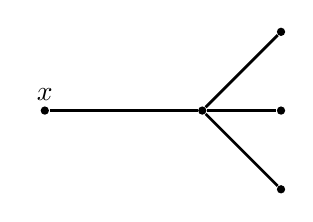
\begin{tikzpicture} 
\draw  node[fill,circle,inner sep=0pt,minimum size=3pt] (n1) at (-1,0) {}
	(-1,0) node [text=black,above] {$x$}
	node[fill,circle,inner sep=0pt,minimum size=3pt] (n2) at (1,0) {}
	node[fill,circle,inner sep=0pt,minimum size=3pt] (n6) at (2,1) {}
	node[fill,circle,inner sep=0pt,minimum size=3pt] (n7) at (2,0) {}
	node[fill,circle,inner sep=0pt,minimum size=3pt] (n8) at (2,-1) {};
	
\draw [line width = 1 pt, black, -] (n1) edge node {} (n2) 

[line width = 1 pt, black, -] (n2) edge node {} (n6)
[line width = 1 pt, black, -] (n2) edge node {} (n7)
[line width = 1 pt, black, -] (n2) edge node {} (n8);
\end{tikzpicture}
\end{center}
\begin{align*}
P_G(t)=P_{G-x}(t)(t-1) = t(t-1)^{n-2}(t-1)=t(t-1)^{n-1}
\end{align*}
by induction.
\end{proof}
\begin{lemma}
For the disjoint union of graphs $G,H$, $P(G\sqcup H,t) =P(G,t)P(H,t) $
\end{lemma}
\begin{proof}
Any pair (colouring of $G$, colouring of $H$) gives a colouring of $G\sqcup H$.
\end{proof}
The chromatic function is indeed the chromatic polynomial.
\begin{proposition}
For a graph $G\neq \emptyset$, let $\pi_i(G)$ be the number of ways to partition $V(G)$ into exactly $i$ non-empty independent sets. Then
\begin{align*}
P_G(t)=\sum_{i=0}^n \pi_i(G) t^{\underline{i}}\quad ,\qquad n=|V(G)|
\end{align*}
\end{proposition}
\begin{proof}
The choice of a colouring with colours from $\lbrace 1,\dots , t\rbrace$ is the same as 
\begin{enumerate}
\item[$\circ$] partitioning into $i$ independent sets: $\pi_i(G)$ ways to do this.
\item[$\circ$] colouring each part with a different colour: $t(t-1) \cdots  (t-(i-1))=t^{\underline{i}}$ ways.
\end{enumerate}
And we do this for $1\le i \le n$
\end{proof}
\begin{example}
Let $G=P_3$. \begin {tikzpicture}
\draw 
node[fill,circle,inner sep=0pt,minimum size=3pt] (n1) at (0,0) {}
(0,0) node [text=black,above] {$1$}
[line width = 1 pt, black, -] (n1) edge node {} (n2)
node[fill,circle,inner sep=0pt,minimum size=3pt] (n2) at (1,0) {}
(1,0) node [text=black,above] {$2$}
node[fill,circle,inner sep=0pt,minimum size=3pt] (n3) at (2,0) {}
(2,0) node [text=black,above] {$3$}
[line width = 1 pt, black, -] (n1) edge node {} (n3);
\end {tikzpicture}
\begin{align*}
\pi_1 &=0\\
\pi_2 &= 1\quad ,\qquad 1-2-1\\
\pi_3 &= 1\quad ,\qquad 1-2-3\\
\pi_{\ge 4} &= 0
\end{align*}
Then
\begin{align*}
P_{P_3}(t)=\pi_2t^{\underline{2}}+\pi_3 t^{\underline{3}}=t(t-1)+t(t-1)(t-2)=t(t-1)^2
\end{align*}
\end{example}
\begin{remark}
Hence from now on we call $P_G(t)$ the chromatic polynomial.
\end{remark}
\begin{proposition}
$G=(V,E)$ is a graph. If $G\neq \emptyset$, then
\begin{align*}
P_G(t)=\sum_{F\subseteq E} (-1)^{|F|} t^{c(F)}
\end{align*}
where $c(F)$ is the number of connected components of $(V,F)$.
\end{proposition}
Before the proof we remind ourselves of the Inclusion-Exclusion principle.
\begin{fact}
Suppose $A$ is a set, and $A_1,\dots , A_k$ are subsets of $A$. For any $X\subseteq \lbrace 1,\dots , k\rbrace$ define
\begin{align*}
A_X=\bigcap_{i\in X} A_i
\end{align*}
Then
\begin{align*}
\left| \overline{\bigcup_{i=1}^k A_i}\right| = \sum_{X\subseteq \lbrace 1,\dots , k\rbrace} (-1)^{|X|}|A_X|
\end{align*}
\end{fact}
\begin{example} Assume we have some ambient set $\mathcal{A}$, with  $A,B,C \subset \mathcal{A}$.\\
\def\firstcircle{(0,0) circle (1.5cm)}
\def\secondcircle{(60:2cm) circle (1.5cm)}
\def\thirdcircle{(0:2cm) circle (1.5cm)}
\begin{center}
\begin{tikzpicture}
    \begin{scope}[shift={(3cm,-5cm)}, fill opacity=0.5]
        \fill[red] \firstcircle;
        \fill[green] \secondcircle;
        \fill[blue] \thirdcircle;
        \draw \firstcircle node[below] {$A$};
        \draw \secondcircle node [above] {$B$};
        \draw \thirdcircle node [below] {$C$};
    \end{scope}
\end{tikzpicture}
\end{center}
Then we have
\begin{align*}
|A\cup B \cup C| &= |A|+|B|+|C| -|A\cap B|-|B\cap C|-|C\cap A| + |A\cap B\cap C|\\\\
|\overline{A\cup B\cup C}|&= |\mathcal{A} | - |A|-|B|-|C| +|A\cap B|+|B\cap C|+|A\cap C| -|A\cap B\cap C|
\end{align*}
\end{example}
\begin{proof}[Proof of proposition 9.]
Define $A=\lbrace g:V\to \lbrace 1,\dots ,t\rbrace\rbrace$ - all functions, not just colourings. For every $e=xy\in E$, let $A_e=\lbrace g\in A : g(x)=g(y)\rbrace$. Now for $F\subseteq E$, let $A_F= \bigcap_{e\in F} A_e$. Clearly $|A_F|=t^{c(F)}$, because $g\in A_F$ must be constant on every component of $(V,F)$. But then we're done, as 
\begin{align*}
P_G(t)= \left| \overline{\bigcup_{e\in E} A_e}\right| \overset{Incl.-excl.}{=} \sum_{F\subseteq E} (-1)^{|F|} |A_F|
\end{align*}
\end{proof}
\begin{notation}
If $P(t)$ is a polynomial, we write $[t^k]P(t)$ for the coefficient of $t^k$ in $P(t)$.
\end{notation}
\begin{lemma}
If $G$ is a graph with $n$ vertices and $m$ edges, then $P_G(t)$ is a polynomial of degree $n$, with
\begin{align*}
[t^n]P_G(t)=1\quad , \qquad [t^{n-1}]P_G(t)=-m
\end{align*}
\end{lemma}
\begin{proof}
By proposition 9, we have $c(F)\le n \Rightarrow \deg P_G \le n$. Now then $c(F)=n $ iff. $F=\emptyset$, which implies $t^n$ appears exactly once in $P_G(t)$ with coefficient $(-1)^{|\emptyset|}=1$.\\
$c(F)=n-1$ iff. $F=\lbrace e\rbrace$, which implies $t^{n-1}$ appears with coefficient $(-1)^{-1}m=-m$.
\end{proof}
\begin{notation}
For $e\in E(G)$ we write: $G-e$ for $G$ with $e$ removed, and $G/e$ for $G$ with $e$ contracted. \\
\begin{center}
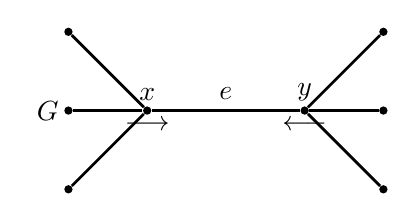
\begin{tikzpicture} 
\draw  node[fill,circle,inner sep=0pt,minimum size=3pt] (n1) at (-1,0) {}
(-1,0) node [text=black,above] {$x$}
(-1,0) node [text=black,below] {$\longrightarrow$}
	node[fill,circle,inner sep=0pt,minimum size=3pt] (n2) at (1,0) {}
	(1,0) node [text=black,above] {$y$}
	(1,0) node [text=black,below] {$\longleftarrow$}
		node[fill,circle,inner sep=0pt,minimum size=3pt] (n3) at (-2,1) {} 
	node[fill,circle,inner sep=0pt,minimum size=3pt] (n4) at (-2,0) {} 
	(-2,0) node [text=black,left] {$G$}
	node[fill,circle,inner sep=0pt,minimum size=3pt] (n5) at (-2,-1) {}
	node[fill,circle,inner sep=0pt,minimum size=3pt] (n6) at (2,1) {}
	node[fill,circle,inner sep=0pt,minimum size=3pt] (n7) at (2,0) {}
	node[fill,circle,inner sep=0pt,minimum size=3pt] (n8) at (2,-1) {};
	
\draw [line width = 1 pt, black, -] (n1) edge node {} (n2) (0,0) node [above] {$e$}
[line width = 1 pt, black, -] (n1) edge node {} (n3)
[line width = 1 pt, black, -] (n1) edge node {} (n4)
[line width = 1 pt, black, -] (n1) edge node {} (n5)
[line width = 1 pt, black, -] (n2) edge node {} (n6)
[line width = 1 pt, black, -] (n2) edge node {} (n7)
[line width = 1 pt, black, -] (n2) edge node {} (n8);
\end{tikzpicture}
\end{center}
\begin{center}
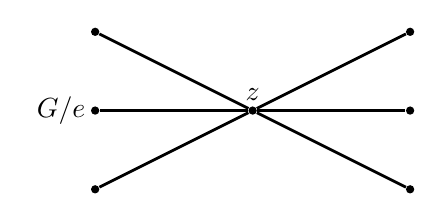
\begin{tikzpicture} 
\draw  
	node[fill,circle,inner sep=0pt,minimum size=3pt] (n1) at (0,0) {}
	(0,0) node [text=black,above] {$z$}
		node[fill,circle,inner sep=0pt,minimum size=3pt] (n3) at (-2,1) {} 
	node[fill,circle,inner sep=0pt,minimum size=3pt] (n4) at (-2,0) {} 
		(-2,0) node [text=black,left] {$G/e$}
	node[fill,circle,inner sep=0pt,minimum size=3pt] (n5) at (-2,-1) {}
	node[fill,circle,inner sep=0pt,minimum size=3pt] (n6) at (2,1) {}
	node[fill,circle,inner sep=0pt,minimum size=3pt] (n7) at (2,0) {}
	node[fill,circle,inner sep=0pt,minimum size=3pt] (n8) at (2,-1) {};
	
\draw 
[line width = 1 pt, black, -] (n1) edge node {} (n3)
[line width = 1 pt, black, -] (n1) edge node {} (n4)
[line width = 1 pt, black, -] (n1) edge node {} (n5)
[line width = 1 pt, black, -] (n1) edge node {} (n6)
[line width = 1 pt, black, -] (n1) edge node {} (n7)
[line width = 1 pt, black, -] (n1) edge node {} (n8);
\end{tikzpicture}
\end{center}
\end{notation}
\begin{proposition}
(Deletion-contraction rule). If $e\in E(G)$, then
\begin{align*}
P_G(t)=P_{G-e}(t)-P_{G/e}(t)
\end{align*}
\end{proposition}
\begin{proof}
Let $e=xy\in E(G)$.
\begin{align*}
P_{G-e}(t)&=\#\text{ colourings with } c(x)\neq c(y) + \# \text{ colourings with } c(x)=c(y) \\
&= P_G(t)+P_{G/e}(t)
\end{align*}
\end{proof}
\begin{remark}
$|E(G-e)|=|E(G)|-1$ and $|V(G/e)|=|V(G)|-1$, so we could define $P_G(t)$ recursively
\begin{align*}
P_G(t) = \left\lbrace \begin{array}{ll}
t^{|V(G)|} & \text{if } G \text{ has no edges}\\
 & \\
P_{G-e}(t)-P_{G/e}(t) & \text{if } e\in E(G)
\end{array} \right.
\end{align*}
\end{remark}
\begin{example} $G$ is a graph on $5$ vertices, and we run the above.\\
\begin{center}
\begin {tikzpicture}
\draw
node[fill,circle,inner sep=0pt,minimum size=3pt] (n1) at (0,1) {}

node[fill,circle,inner sep=0pt,minimum size=3pt] (n2) at (1.25,0) {}

node[fill,circle,inner sep=0pt,minimum size=3pt] (n3) at (0.75,-1) {}

node[fill,circle,inner sep=0pt,minimum size=3pt] (n4) at (-0.75,-1) {}

node[fill,circle,inner sep=0pt,minimum size=3pt] (n5) at (-1.25,0) {}

	(1.5,0) node [text=black,right] {$=$} 
[line width = 1 pt, black, -] (n1) edge (n2)
[line width = 1 pt, black, -] (n2) edge (n3)
[line width = 1 pt, black, -] (n3) edge (n4)
[line width = 1 pt, black, -] (n4) edge (n5)
[line width = 1 pt, black, -] (n5) edge (n1)
[line width = 1 pt, black, -] (n1) edge (n4)
[line width = 1 pt, black, -] (n1) edge (n3)
; 
\end {tikzpicture}
\begin {tikzpicture}
\draw
node[fill,circle,inner sep=0pt,minimum size=3pt] (n1) at (0,1) {}

node[fill,circle,inner sep=0pt,minimum size=3pt] (n2) at (1.25,0) {}

node[fill,circle,inner sep=0pt,minimum size=3pt] (n3) at (0.75,-1) {}

node[fill,circle,inner sep=0pt,minimum size=3pt] (n4) at (-0.75,-1) {}

node[fill,circle,inner sep=0pt,minimum size=3pt] (n5) at (-1.25,0) {}

	(1.5,0) node [text=black,right] {$-$} 
[line width = 1 pt, black, -] (n1) edge (n2)
[line width = 1 pt, black, -] (n2) edge (n3)

[line width = 1 pt, black, -] (n4) edge (n5)
[line width = 1 pt, black, -] (n5) edge (n1)
[line width = 1 pt, black, -] (n1) edge (n4)
[line width = 1 pt, black, -] (n1) edge (n3)
; 
\end {tikzpicture}
\begin {tikzpicture}
\draw
node[fill,circle,inner sep=0pt,minimum size=3pt] (n1) at (0,1) {}

node[fill,circle,inner sep=0pt,minimum size=3pt] (n2) at (1,0) {}

node[fill,circle,inner sep=0pt,minimum size=3pt] (n3) at (0,-1) {}

node[fill,circle,inner sep=0pt,minimum size=3pt] (n5) at (-1,0) {}


[line width = 1 pt, black, -] (n1) edge (n2)
[line width = 1 pt, black, -] (n2) edge (n3)
[line width = 1 pt, black, -] (n5) edge (n1)
[line width = 1 pt, black, -] (n1) edge (n3)
[line width = 1 pt, black, -] (n3) edge (n5)
; 
\end {tikzpicture}
\end{center}
\begin{center}
\begin {tikzpicture}
\draw
node[fill,circle,inner sep=0pt,minimum size=3pt] (n1) at (0,1) {}

node[fill,circle,inner sep=0pt,minimum size=3pt] (n2) at (1.25,0) {}

node[fill,circle,inner sep=0pt,minimum size=3pt] (n3) at (0.75,-1) {}

node[fill,circle,inner sep=0pt,minimum size=3pt] (n4) at (-0.75,-1) {}

node[fill,circle,inner sep=0pt,minimum size=3pt] (n5) at (-1.25,0) {}
	(-1.5,0) node [text=black,left] {$=$} 
	(1.5,0) node [text=black,right] {$-$} 
[line width = 1 pt, black, -] (n1) edge (n2)
[line width = 1 pt, black, -] (n2) edge (n3)

[line width = 1 pt, black, -] (n4) edge (n5)

[line width = 1 pt, black, -] (n1) edge (n4)
[line width = 1 pt, black, -] (n1) edge (n3)
; 
\end {tikzpicture}
\begin {tikzpicture}
\draw
node[fill,circle,inner sep=0pt,minimum size=3pt] (n1) at (0,1) {}

node[fill,circle,inner sep=0pt,minimum size=3pt] (n2) at (1.25,0) {}

node[fill,circle,inner sep=0pt,minimum size=3pt] (n3) at (0.75,-1) {}

node[fill,circle,inner sep=0pt,minimum size=3pt] (n4) at (-0.75,-1) {}

	(1.5,0) node [text=black,right] {$-$} 
[line width = 1 pt, black, -] (n1) edge (n2)
[line width = 1 pt, black, -] (n2) edge (n3)



[line width = 1 pt, black, -] (n1) edge (n4)
[line width = 1 pt, black, -] (n1) edge (n3)
; 
\end {tikzpicture}
\begin {tikzpicture}
\draw
node[fill,circle,inner sep=0pt,minimum size=3pt] (n1) at (0,1) {}

node[fill,circle,inner sep=0pt,minimum size=3pt] (n2) at (1,0) {}

node[fill,circle,inner sep=0pt,minimum size=3pt] (n3) at (0,-1) {}

node[fill,circle,inner sep=0pt,minimum size=3pt] (n5) at (-1,0) {}

	(1.5,0) node [text=black,right] {$+$} 
[line width = 1 pt, black, -] (n1) edge (n2)
[line width = 1 pt, black, -] (n2) edge (n3)

[line width = 1 pt, black, -] (n1) edge (n3)
[line width = 1 pt, black, -] (n3) edge (n5)
; 
\end {tikzpicture}
\begin {tikzpicture}
\draw
node[fill,circle,inner sep=0pt,minimum size=3pt] (n1) at (0,1) {}

node[fill,circle,inner sep=0pt,minimum size=3pt] (n3) at (0,-1) {}

node[fill,circle,inner sep=0pt,minimum size=3pt] (n5) at (-1,0) {}


[line width = 1 pt, black, -] (n1) edge (n3)
[line width = 1 pt, black, -] (n3) edge (n5)
[line width = 1 pt, black, -] (n5) edge (n1)
; 
\end {tikzpicture}
\end{center}
Now arrange the graphs accordingly s.t.
\begin{center}
\begin {tikzpicture}
\draw
node[fill,circle,inner sep=0pt,minimum size=3pt] (n1) at (-2,0) {}
	(-2,0) node [text=black,above] {$t-1$}
node[fill,circle,inner sep=0pt,minimum size=3pt] (n2) at (-1,0) {}
	(-1,0) node [text=black,above] {$t-1$}
node[fill,circle,inner sep=0pt,minimum size=3pt] (n3) at (0,0) {}
	(0,-.25) node [text=black,below] {$t-2$}
node[fill,circle,inner sep=0pt,minimum size=3pt] (n4) at (1,-1) {}
	(1,-1) node [text=black,right] {$t-1$}
node[fill,circle,inner sep=0pt,minimum size=3pt] (n5) at (1,1) {}
	(1,1) node [text=black,right] {$t$}
	(-3,0) node [text=black,left] {$=$} 
	(1.5,0) node [text=black,right] {$-$} 

[line width = 1 pt, black, -] (n1) edge (n2)
[line width = 1 pt, black, -] (n2) edge (n3)
[line width = 1 pt, black, -] (n3) edge (n4)
[line width = 1 pt, black, -] (n3) edge (n5)
[line width = 1 pt, black, -] (n4) edge (n5); 
\end {tikzpicture}
\begin {tikzpicture}
\draw
node[fill,circle,inner sep=0pt,minimum size=3pt] (n2) at (-1,0) {}
	(-1,0) node [text=black,above] {$t-1$}
node[fill,circle,inner sep=0pt,minimum size=3pt] (n3) at (0,0) {}
	(0,-.25) node [text=black,below] {$t-2$}
node[fill,circle,inner sep=0pt,minimum size=3pt] (n4) at (1,-1) {}
	(1,-1) node [text=black,right] {$t-1$}
node[fill,circle,inner sep=0pt,minimum size=3pt] (n5) at (1,1) {}
	(1,1) node [text=black,right] {$t$}
	(-2,0) node [text=black,left] {$2\times $} 
	(1.5,0) node [text=black,right] {$+$} 


[line width = 1 pt, black, -] (n2) edge (n3)
[line width = 1 pt, black, -] (n3) edge (n4)
[line width = 1 pt, black, -] (n3) edge (n5)
[line width = 1 pt, black, -] (n4) edge (n5); 
\end {tikzpicture}
\begin {tikzpicture}
\draw
node[fill,circle,inner sep=0pt,minimum size=3pt] (n3) at (0,0) {}
	(0,0) node [text=black,left] {$t-2$}
node[fill,circle,inner sep=0pt,minimum size=3pt] (n4) at (1,-1) {}
	(1,-1) node [text=black,right] {$t-1$}
node[fill,circle,inner sep=0pt,minimum size=3pt] (n5) at (1,1) {}
	(1,1) node [text=black,right] {$t$}
 


[line width = 1 pt, black, -] (n3) edge (n4)
[line width = 1 pt, black, -] (n3) edge (n5)
[line width = 1 pt, black, -] (n4) edge (n5); 
\end {tikzpicture}
\end{center}
\begin{align*}
= t(t-1)^3-2t(t-1)^2(t-2)(t-2)+t(t-1)(t-2)
\end{align*}
\end{example}
\begin{example}
$P(C_n,t)=P(P_n,t)-P(C_{n-1},t)$. We have
\begin{align*}
P(P_n,t)&= t(t-1)^{n-1}\\
P(C_3,t)&=t(t-1)(t-2)
\end{align*}
By induction $P(C_n)=(t-1)^n+(-1)^n(t-1)$. We can check that $P(C_n,2)\neq 0$ iff. $2|n$.
\begin{align*}
P(C_n,2)=1+(-1)^2= \left\lbrace \begin{array}{ll}
2, & 2\mid n\\
0, & 2\nmid n
\end{array}\right.
\end{align*}
\end{example}
\begin{proposition}
Let $G\neq \emptyset$ be a graph with $n$ vertices, $m$ edges and $c$ connected components. The coefficients of $P_G(t)$ alternate in signs, i.e.
\begin{align*}
P_G(t)=\sum_{i=0}^n (-1)^i c_i(G)t^{n-i}
\end{align*}
where $c_i(G)\ge 0$. Moreover $c_i(G)=0$ for $i>n-c$ and $c_{n-c}(G)\neq 0$.
\end{proposition}
\underline{Simply put:}
\begin{align*}
P_G(t)=t^n-mt^{n-1}+c_2(G)t^{n-2}-\cdots + (-1)^{n-c}c_{n-c}(G)t^c
\end{align*}
the last term $t^c$ is with $t$ to the power of the number of connected components. Exercise: do a proof by induction.
\begin{proof} Deleting keeps the sign, and contracting changes the sign.\\
\begin{center}
\begin {tikzpicture}
\draw
node[fill,circle,inner sep=0pt,minimum size=3pt] (n1) at (0,2) {}
	(0,2) node [text=black,above] {$G$}
node[fill,circle,inner sep=0pt,minimum size=3pt] (n2) at (-2,0) {}
	(-2,0) node [text=black,left] {$G'$}
node[fill,circle,inner sep=0pt,minimum size=3pt] (n3) at (2,0) {}
	(2,0) node [text=black,right] {$G''$}
node[fill,circle,inner sep=0pt,minimum size=3pt] (n4) at (-3,-2) {}
node[fill,circle,inner sep=0pt,minimum size=3pt] (n5) at (-1,-2) {}
node[fill,circle,inner sep=0pt,minimum size=3pt] (n6) at (1,-2) {}
node[fill,circle,inner sep=0pt,minimum size=3pt] (n7) at (3,-2) {}
node[fill,circle,inner sep=0pt,minimum size=0pt] (n8) at (-3,-2.5) {}
node[fill,circle,inner sep=0pt,minimum size=0pt] (n9) at (-1,-2.5) {}
node[fill,circle,inner sep=0pt,minimum size=0pt] (n10) at (1,-2.5) {}
node[fill,circle,inner sep=0pt,minimum size=0pt] (n11) at (3,-2.5) {}

[line width = 1 pt, black, -] (n1) edge (n2)
(-1,1) node [left] {$G-e$}
(-2,0) node [right] {$\cdot 1$}
[line width = 1 pt, black, -] (n1) edge (n3)
(1,1) node [right] {$G/e$}
(2,0) node [left] {$\cdot (-1)$}
[line width = 1 pt, black, -] (n2) edge (n4)
(-2.5,-1) node [left] {$G-e$}
(-3,-2) node [left] {$\cdot 1$}
[line width = 1 pt, black, -] (n2) edge (n5)
(-1.5,-1) node [right] {$G/e$}
(-1,-2) node [right] {$\cdot (-1)$}
[line width = 1 pt, black, -] (n3) edge (n6)
(1.5,-1) node [left] {$G-e$}
(1,-2) node [left] {$\cdot 1$}
[line width = 1 pt, black, -] (n3) edge (n7)
(2.5,-1) node [right] {$G/e$}
(3,-2) node [right] {$\cdot (-1)$}
[line width = 1 pt, black, -] (n4) edge (n8)
(-3,-2.5) node [below] {$\overline{K_i}$}
[line width = 1 pt, black, -] (n5) edge (n9)
(-1,-2.5) node [below] {$\overline{K_j}$}
[line width = 1 pt, black, -] (n6) edge (n10)
[line width = 1 pt, black, -] (n7) edge (n11)
; 
\end {tikzpicture}
\end{center}
Every branch of the deletion-contraction tree ends with some $\overline{K_i}$, $1\le i \le n$. Every branch ending with $\overline{K_i}$ contributes
\begin{align*}
(-1)^{n-i}t^i
\end{align*}
because the path from $G$ to $\overline{K_i}$ contains $n-i$ contractions, i.e. $n-i$ sign changes. The proposition holds with
\begin{align*}
c_i(G)=\# \text{ of branches ending with } \overline{K_i}
\end{align*}
and clearly $c_i(G)\geq 0$.

To prove that $c_i(G)=0$ for $i>n-c$ note no branch of the tree ends with with a graph on less than $c$ vertices. Moreover, there is at least one branch with ends exactly with $K_c$ (apply contractions all the time), so $c_{n-c}(G)>0$.
\end{proof}

\end{document}




